\documentclass[12pt,compress,aspectratio=169]{beamer}

\usetheme{metropolis}
\setbeamersize{text margin left=.5cm,text margin right=.5cm}

%\usepackage[utf8]{inputenc}
\usefonttheme{professionalfonts}
\usepackage{amsmath}
\usepackage{siunitx}
%\usepackage{graphicx}
\usepackage{tikz}
\usepackage{mathpazo}
%\usepackage[scaled]{helvet}
\usepackage{bm}
%\usepackage{xcolor,colortbl}
%\usepackage{hyperref}

\sisetup{
  detect-all,
  math-sf=\textsf,
  per-mode=symbol
}

\setsansfont{Roboto Light}
\setmonofont{Ubuntu Mono}
\setlength{\parskip}{0pt}
\renewcommand{\baselinestretch}{1}


\title{Topic 1: Kinematics}
\subtitle{Advanced Placement Physics C}
\author[TML]{Dr.\ Timothy Leung}
\institute{Olympiads School}
\date{\today}


\newcommand{\iii}{\ensuremath\hat{\bm{\imath}}}
\newcommand{\jjj}{\ensuremath\hat{\bm{\jmath}}}
\newcommand{\kkk}{\ensuremath\hat{\bm{k}}}
\newcommand{\pic}[2]{\includegraphics[width=#1\textwidth]{#2}}
\newcommand{\mb}[1]{\ensuremath\mathbf{#1}}
\newcommand{\eq}[2]{\vspace{#1}{\Large\begin{displaymath}#2\end{displaymath}}}
\newcommand{\magdir}[2]{#1\text{ [#2]}}

\begin{document}

\begin{frame}{}

  {\LARGE
    \begin{center}
      \textbf{WELCOME TO AP PHYSICS C}
    \end{center}
  }
\end{frame}



\begin{frame}{Pre-requisites}
  \begin{itemize}
  \item\textbf{Physics 11 and 12:} You will need to be comfortable with the
    topics covered in high-school level physics courses.
  \item\textbf{Calculus:} Physics C exams are calculus based, and you will be
    required to do basic differentiation and integration. You don't need to be
    an expert, but basic knowledge is required. Differentiation and integration
    in the course are generally not difficult, but there are occasional
    challenges.
  \item\textbf{Vectors:} You need to be comfortable with vector operations,
    including addition and subtraction, multiplication/division by constants,
    as well as dot products and cross products.
  \end{itemize}
\end{frame}



\begin{frame}{AP Physics C Exams}
  There are calculus-based 2 AP Physics C exams, which are usually taken
  together on the same day, in the first or second week of May of each year.
  \begin{itemize}
  \item Mechanics
  \item Electricity and Magnetism
  \end{itemize}
\end{frame}



\begin{frame}{Classroom Rules}
  \begin{itemize}
  \item Treat each other with respect
  \item Raise your hands if you have a question. Don't wait too long
  \item E-mail me at \texttt{tleung@olympiadsmail.ca} for any questions related
    to physics and math and engineering
  \item Do \textbf{\emph{not}} try to find me on social media
  \end{itemize}
\end{frame}



\begin{frame}
  \titlepage
\end{frame}



\begin{frame}{Files for You to Download}
  There are a considerable number of files for you to download at the beginning
  of the course:
  \begin{itemize}
  \item\texttt{PhysAPC-courseOutline.pdf}--The course outline
  \item\texttt{PhysAPC-equationSheet.pdf}--Equation sheet for your exams
  \item\texttt{PhysAPC-01-kinematics.pdf}
  \item\texttt{PhysAPC-01a-vectorCalculus.pdf}--Vectors and calculus handout
  \item\texttt{PhysAPC-01b-kinematicsHandout.pdf}--Basic kinematics, expanded
    version
  \item\texttt{PhysAPC-01c-motionGraphs.pdf}--Handout on motion graphs
  %\item\texttt{PhysAPC-01e-projectileMotion.pdf}--Handout on projectile motion
  %\item\texttt{PhysAPC-02-dynamics.pdf}
  \item\texttt{PhysAPC-01-Homework.pdf}--Homework problems for Topic 1
  %\item\texttt{PhysAPC-02-Homework.pdf}--Homework problems for Topic 2
  \end{itemize}
\end{frame}


\begin{frame}{File Download}
  Please download/print the PDF file for the class slides before
  each class. There is no point copying notes that are already on the slides.
  Instead, focus on things that aren't necessarily on the slides. If you wish
  to print the slides, we recommend printing \emph{four} slides per page.
\end{frame}



\begin{frame}{Vectors and Calculus}
  Please refer to the handout to make sure that you are familiar with
  basic vector and calculus.
\end{frame}



\section{Kinematics}

\begin{frame}{Kinematics}
  \textbf{Kinematics} is a discipline within mechanics concerning the
  motion of bodies. It describes the relationship between 
  \begin{itemize}
  \item<alert@1> Position
  \item<alert@1> Displacement
  \item Distance 
  \item<alert@1> Velocity
  \item Speed
  \item<alert@1> Acceleration
  \end{itemize}
  Kinematics does not deal with the causes of motion.
\end{frame}



\begin{frame}{Position}
  \textbf{Position} $\mb{x}$ describes the location of an object in a
  coordinate system.%\footnote{The coordinate system is usually
  %\emph{Cartesian}, but it can also be \emph{polar}, \emph{cylindrical} or
  %\emph{spherical}}.
  The origin of the coordinate system is called the ``reference point''.
  The SI unit for position is \textbf{meter}, \si{\metre}.
  
  \eq{-.2in}{
    \boxed{\mb{x}(t)=x(t)\iii + y(t)\jjj + z(t)\kkk}
  }

  Vectors in 2D/3D Cartesian space are generally using the
  \textbf{IJK notation}
  \begin{itemize}
  \item $\iii$, $\jjj$ and $\kkk$ are \textbf{basis vectors} indicating the
    directions of the $x$, $y$ and $z$ axes. Basis vectors are
    \textbf{unit vectors} (i.e.\ length $1$)
  \item The IJK notation does not explicitly give the magnitude or the direction
    of the vector (needs to be calculated using the Pythagorean theorem)
  \end{itemize}
\end{frame}



\begin{frame}{Displacement}
  \textbf{Displacement} $\Delta\mb{x}(t)$ is the change in position from the
  initial position $\mb{x}_0$ within the same coordinate system:

  \eq{-.25in}{
    \boxed{
      \Delta\mb{x}(t)=\mb{x}(t)-\mb{x}_0
      =(x-x_0)\iii + (y-y_0)\jjj + (z-z_0)\kkk
    }
  }
  \begin{itemize}
  \item IJK notation makes vector addition and subtraction less prone to errors
  \item Since the reference point $\mb{x}_{\textrm{ref}}=\mb{0}$, the position
    vector $\mb{x}$ is also its displacement from the reference point
  \end{itemize}
\end{frame}


\begin{frame}{Distance}
  \textbf{Distance} $s(t)$ is a quantity that is \emph{related} to displacement.
  The unit for distance is also a meter (\si{\metre}).
  \begin{columns}
    \column{.7\textwidth}
    \begin{itemize}
    \item The length of the path taken by an object when it travels from
      $\mb{x}_0$ to $\mb{x}$
    \item A scalar quantity
    \item Always positive, i.e.\ $s\geq 0$
    \item Although the magnitude of the displacement vector is also a scalar,
      it is not necessarily the same as distance
    \item $s\geq |\Delta\mb{x}|$
    \end{itemize}
    
    \column{.3\textwidth}
    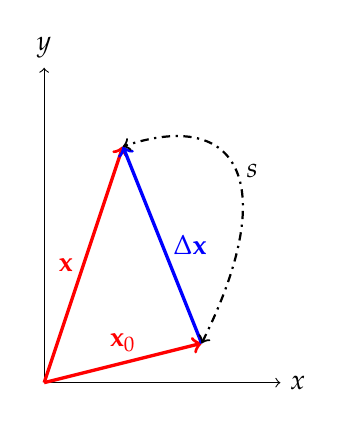
\begin{tikzpicture}[scale=.5]
      \draw[->](0,0)--(6,0) node[pos=1,right]{$x$};
      \draw[->](0,0)--(0,8) node[pos=1,above]{$y$};
      \draw[->,red,very thick] (0,0)--(4,1) node[midway,above]{$\mb{x}_0$};
      \draw[->,red,very thick] (0,0)--(2,6) node[midway,left]{$\mb{x}$};
      \draw[->,blue,very thick](4,1)--(2,6) node[midway,right]{$\Delta\mb{x}$};
      \draw[thick,dash dot,<->] (4,1)..controls (6,5) and (5,7)..(2,6)
      node[midway,right]{$s$};
    \end{tikzpicture}
  \end{columns}
\end{frame}



\begin{frame}{Instantaneous Velocity}
  If position $\mb{x}$ is differentiable in time $t$, then velocity
  can be found at any time $t$. The \textbf{instantaneous velocity}
  $\mb{v}(t)$ of an object is the time rate of change of position. The unit for
  velocity is \textbf{meters per second} (\si{\metre\per\second}):

  \eq{-.2in}{
    \boxed{
      \mb{v}(t)= \frac{d\mb{x}}{dt}
    }
  }
  
  Since $\mb{x}$ has $x$, $y$ and $z$ components along the $\iii$, $\jjj$ and
  $\kkk$ directions (linearly independent), we can take the time derivative in
  every component:

  \eq{-.15in}{
    \mb{v}(t)= \frac{d\mb{x}}{dt}=
    \frac{dx}{dt}\iii + \frac{dy}{dt}\jjj + \frac{dz}{dt}\kkk =
    u\iii + v\jjj + w\kkk
  }
\end{frame}



\begin{frame}{Integrating Velocity to Get Position/Displacement}
  Conversely, if $\mb{v}(t)$ is the time rate of change of position
  $\mb{x}(t)$, then $\mb{x}(t)$ is the time integral of $\mb{v}(t)$:
  
  \eq{-.2in}{
    \boxed{
      \mb{x}(t)=\int\mb{v}(t)dt + \mb{x}_0
    }
  }
  
  The constant of integration $\mb{x}_0$ is the \emph{initial position} at
  $t=\num{0}$. We can integrate each component to get $\mb{x}$:

 \eq{-.2in}{ \mb{x}(t)= \left(
    \int u\iii + \int v\jjj + \int w\kkk \right) dt + \mb{x}_0
  }
\end{frame}



\begin{frame}{Average Velocity}
  \textbf{Average velocity} $\overline{\mb{v}}$ of an object is the finite
  change in position $\Delta\mb{x}$ over a \emph{finite} time interval
  $\Delta t$:

  \eq{-.3in}{
    \boxed{
      \overline{\mb{v}}= \frac{\Delta\mb{x}}{\Delta t}
    }
  }
  
  Like instantaneous velocity, we can find the $x$, $y$ and $z$ components of
  average velocity by separating components in each direction:

  \eq{-.15in}{
    \overline{\mb{v}}=
    \frac{\Delta x}{\Delta t}\iii+
    \frac{\Delta y}{\Delta t}\jjj+
    \frac{\Delta z}{\Delta t}\kkk
  }

  (The notation $\overline{v}$ means that $v$ is averaged over \emph{time},
  while the notation $\langle v\rangle$ is used if $v$ is the average of
  many particles (called an \emph{ensemble average})
\end{frame}



\begin{frame}{Instantaneous \& Average Speed}
  \textbf{Instantaneous speed} $v$ is the time rate of change of
  \emph{distance}:

  \eq{-.2in}{
    \boxed{
      v=\frac{ds}{dt}
    }
  }
  \begin{itemize}
  \item\vspace{-.1in}Since %distance of \emph{any} path is always positive
    $s\geq 0$, instantaneous speed must also be positive $v\geq 0$
  \item Instantaneous speed is the magnitude of the instantaneous velocity
    vector, i.e.\ $v=|\mb{v}|$
  \end{itemize}
  Likewise, \textbf{average speed} is similar to average velocity: it is the
  distance travelled over a finite time interval.
  
  \eq{-.2in}{
    \boxed{
      \overline{v}=\frac{s}{\Delta t}
    }
  }
\end{frame}



%\begin{frame}{Path}
%  Sometimes instead of explicitly describing the position $x=x(t)$ and $y=y(t)$,
%  the path of an object can be given in terms of $x$ coordinate $y=y(x)$, while
%  giving the $x$ (or $y$) coordinate as a function of time.
%  \begin{itemize}
%  \item In this case, substitute the expression for $x(t)$ into $y=y(x)$ to
%    get an expression of $y=y(t)$
%  \item Take derivative using chain rule to get $v_y=v_y(t)$
%  \end{itemize}
%\end{frame}


\begin{frame}{Instantaneous \& Average Acceleration}
  In the same way that velocity is the time rate of change in position,
  \textbf{instantaneous acceleration} $\mb{a}(t)$ is the time rate of change in
  velocity, with a unit of \textbf{meters per unit squared}
  (\si{\metre\per\second^2}):

  \eq{-.2in}{
    \boxed{
      \mb{a}(t)= \frac{d\mb{v}}{dt}=\frac{d^2\mb{x}}{dt^2}
    }
  }

  Likewise, \textbf{average acceleration} $\overline{\mb{a}}$ is the finite
  change in velocity $\Delta\mb{v}$ over a finite time interval $\Delta t$:

  \eq{-.25in}{
    \overline{\mb{a}} = \frac{\Delta\mb{v}}{\Delta t}
    =\frac{\mb{v}-\mb{v}_0}{\Delta t}
  }
  
  Note that acceleration only requires a \emph{change} in velocity. It does
  \emph{not} necessarily mean an object has to speed up or slow down.
\end{frame}



\begin{frame}{Special Notation}{When Differentiating With Time}
  Physicists and engineers use a special notation when the derivative is
  taken with respect to \emph{time}, by writing a dot above the variable:
  \begin{itemize}
  \item Velocity:

    \eq{-.25in}{
      \mb{v}(t)= \dot{\mb{x}}
    }
  \item Acceleration:

    \eq{-.25in}{
      \mb{a}(t)= \dot{\mb{v}}=\ddot{\mb{x}}
    }
  \end{itemize}
  We will use this notation whenever it is convenient
\end{frame}



\begin{frame}{Integrating Acceleration to Get Velocity}
  Velocity $\mb{v}(t)$ is the time integral of acceleration $\mb{a}(t)$:
    
  \eq{-.2in}{
    \boxed{
      \mb{v}(t)=\int\mb{a}(t)dt+\mb{v}_0
    }
  }

  Again, we can integrate each component of the vector independently:

  \eq{-.2in}{
    \mb{v}(t)=
    \left(\int a_x\iii + \int a_y\jjj + \int a_z\kkk \right) dt +\mb{v}_0
  }
\end{frame}



\begin{frame}{If You Are Curious}
  The time derivative of acceleration is called \textbf{jerk}, with a unit
  of \si{\metre\per\second^3}:

  \eq{-.2in}{
    \mb{j}=\frac{d\mb{a}}{dt}=\frac{d^2\mb{v}}{dt^2}=\frac{d^3\mb{x}}{dt^3}
  }

  The time derivative of jerk is \textbf{jounce}, or \textbf{snap}, with a
  unit of \si{\metre\per\second^4}:
  
  \eq{-.2in}{
    \mb{s}=\frac{d\mb{j}}{dt}=\frac{d^2\mb{a}}{dt^2}=\frac{d^3\mb{v}}{dt^3}
    =\frac{d^4\mb{x}}{dt^4}
  }
  
  The next two derivatives of snap are called \textbf{crackle} and
  \textbf{pop}, but these higher derivatives of position vector are rarely used.
  We will \emph{not} be using them.
\end{frame}



\begin{frame}{Acceleration as Functions of Velocity and Position}
  Acceleration may be expressed as functions of velocity and position rather
  than of time, if an object's motion is dominated by these forces:
  \begin{itemize}
  \item Gravitational or electrostatic forces:
    $\displaystyle a(x)=\frac{Gm_s}{x^2}\quad a(x)=\frac{kq_1q_2}{mx^2}$
  \item Spring force: $\displaystyle a(x)=-\frac{k}{m}x$
  \item Damping force: $a(v)=-bv$
  \item Aerodynamic drag:
    $\displaystyle a(v)=\left[\frac12\rho C_D A_{\textrm{ref}}\right] v^2$
  \end{itemize}
  In these cases, solving for $x(t)$, $v(t)$ and $a(t)$ will require solving a
  differential equation (see handout).
\end{frame}



\section{Kinematic Equations}

\begin{frame}{Kinematic Equations}
  While kinematic problems in AP Physics C exams often require calculus, these
  basic kinematic equations for \underline{constant acceleration} are still a
  powerful tool.
  \begin{columns}
    \column{.45\textwidth}

    \vspace{-.3in}{\Large
      \begin{align*}
        x &= x_0+ v_0t + \frac12at^2\\
        v &= v_0+at\\
        v^2 &= v_0^2+ 2a(x-x_0)
      \end{align*}
    }
    
    \column{.55\textwidth}
    The variables of interests are:
    \begin{itemize}
    \item Initial position: $x_0$
    \item Position at time $t$: $x$
    \item Initial velocity: $v_0$
    \item Instantaneous velocity: $v$
    \item Acceleration (constant): $a$
    \end{itemize}
  \end{columns}
  Kinematic equations are sometimes called the ``Big-five'' or ``Big-four''
  equations. Here, you will only be given three equations in your equation
  sheet. You will still be required to integrate when acceleration is not
  constant.
\end{frame}



\section{Motion Graphs}

\begin{frame}{Motion Graphs}
  You should already be familiar with the basic motion graphs for 1D motion:
  \begin{itemize}
  \item Position vs.\ time ($x-t$) graph
  \item Velocity vs.\ time ($v-t$) graph
  \item Acceleration vs.\ time ($a-t$) graph
  \end{itemize}

  However, depending on the situation, it may be more useful to plot motion
  using other quantities as well.
\end{frame}



\begin{frame}{Uniform Motion: Constant Velocity}
  \begin{center}
    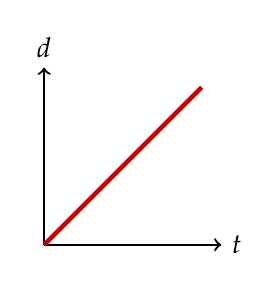
\begin{tikzpicture}[scale=.5]
      \draw[->,thick] (0,0)--(4.5,0) node[pos=1,right]{$t$};
      \draw[->,thick] (0,0)--(0,4.5) node[pos=1,above]{$d$};
      \draw[red!80!black,ultra thick](0,0)--(4,4);
    \end{tikzpicture}
    \hspace{.15in}
    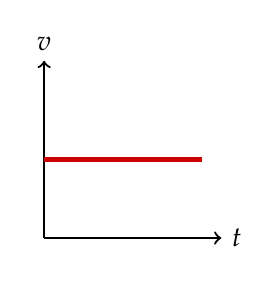
\begin{tikzpicture}[scale=.5]
      \draw[->,thick] (0,0)--(4.5,0) node[pos=1,right]{$t$};
      \draw[->,thick] (0,0)--(0,4.5) node[pos=1,above]{$v$};
      \draw[red!80!black,ultra thick](0,2)--(4,2);
    \end{tikzpicture}
    \hspace{.15in}
    \begin{tikzpicture}[scale=.5]
      \draw[->,thick] (0,0)--(4.5,0) node[pos=1,right]{$t$};
      \draw[->,thick] (0,0)--(0,4.5) node[pos=1,above]{$a$};
      \draw[red!80!black,ultra thick](0,0)--(4,0);
    \end{tikzpicture}
  \end{center}
  \begin{itemize}
  \item Constant velocity has a straight line in the $d-t$ graph
  \item The slope of the $d-t$ graph is the velocity $v$, which is constant
  \item The slope of the $v-t$ graph is the acceleration $a$, which is zero in
    this case
  \end{itemize}
\end{frame}



\begin{frame}{Uniform Acceleration: Constant Acceleration}
  \begin{center}
    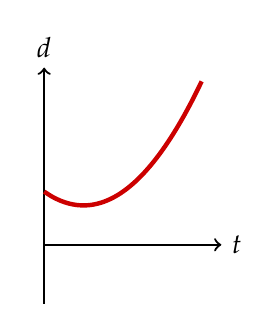
\begin{tikzpicture}[scale=.5]
      \draw[->,thick] (0,0)--(4.5,0) node[pos=1,right]{$t$};
      \draw[->,thick] (0,-1.5)--(0,4.5) node[pos=1,above]{$d$};
      \draw[smooth,samples=20,domain=0:4,red!80!black,ultra thick]
      plot({\x},{0.35*(\x-1)*(\x-1)+1});
    \end{tikzpicture}
    \hspace{.15in}
    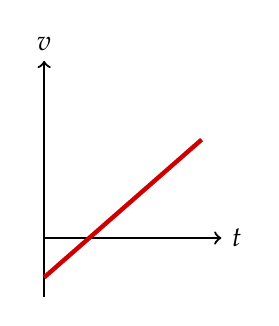
\begin{tikzpicture}[scale=.5]
      \draw[->,thick] (0,0)--(4.5,0) node[pos=1,right]{$t$};
      \draw[->,thick] (0,-1.5)--(0,4.5) node[pos=1,above]{$v$};
      \draw[red!80!black,ultra thick](0,-1)--(4,2.5);
    \end{tikzpicture}
    \hspace{.15in}
    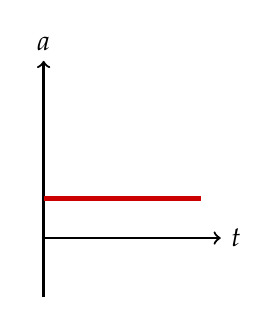
\begin{tikzpicture}[scale=.5]
      \draw[->,thick] (0,0)--(4.5,0) node[pos=1,right]{$t$};
      \draw[->,thick] (0,-1.5)--(0,4.5) node[pos=1,above]{$a$};
      \draw[red!80!black,ultra thick](0,1)--(4,1);
    \end{tikzpicture}
  \end{center}
  \begin{itemize}
  \item The $d-t$ graph for motion with constant acceleration is part of a
    \emph{parabola}
    \begin{itemize}
    \item If the parabola is \emph{convex}, then acceleration is positive
    \item If the parabola is \emph{concave}, then acceleration is negative
    \end{itemize}
  \item The $v-t$ graph is a straight line; its slope (a constant) is the
    acceleration
  \end{itemize}
\end{frame}



\begin{frame}{Simple Harmonic Motion}
  For \textbf{harmonic motions}, neither position, velocity nor acceleration
  are constant:

  \vspace{-.1in}
  \begin{center}
    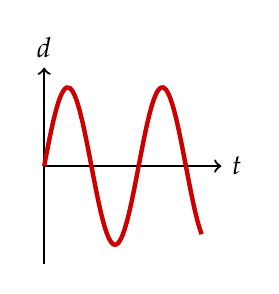
\begin{tikzpicture}[scale=.5]
      \draw[->,thick] (0,0)--(4.5,0) node[pos=1,right]{$t$};
      \draw[->,thick] (0,-2.5)--(0,2.5) node[pos=1,above]{$d$};
      \draw[smooth,samples=50,domain=0:4,red!80!black,ultra thick]
      plot({\x},{2*sin(150*\x)});
    \end{tikzpicture}
    \hspace{.15in}
    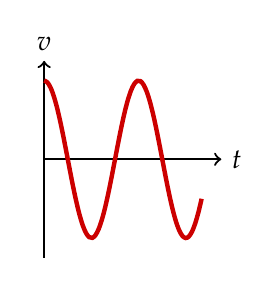
\begin{tikzpicture}[scale=.5]
      \draw[->,thick] (0,0)--(4.5,0) node[pos=1,right]{$t$};
      \draw[->,thick] (0,-2.5)--(0,2.5) node[pos=1,above]{$v$};
      \draw[smooth,samples=50,domain=0:4,red!80!black,ultra thick]
      plot({\x},{2*cos(150*\x)});
    \end{tikzpicture}
    \hspace{.15in}
    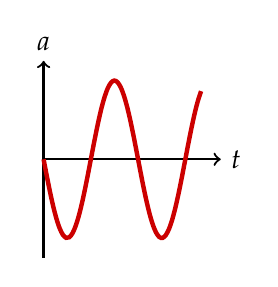
\begin{tikzpicture}[scale=.5]
      \draw[->,thick] (0,0)--(4.5,0) node[pos=1,right]{$t$};
      \draw[->,thick] (0,-2.5)--(0,2.5) node[pos=1,above]{$a$};
      \draw[smooth,samples=50,domain=0:4,red!80!black,ultra thick]
      plot({\x},{-2*sin(150*\x)});
    \end{tikzpicture}
  \end{center}
  Bottom line: regardless of the type motion,
  \begin{itemize}
  \item The $v-t$ graph is the slope of the $d-t$ graph
  \item The $a-t$ graph is the slope of the $v-t$ graph
  \end{itemize}
\end{frame}



\begin{frame}{Area Under Motion Graphs}
  \begin{columns}
    \column{.25\textwidth}
    \begin{center}
      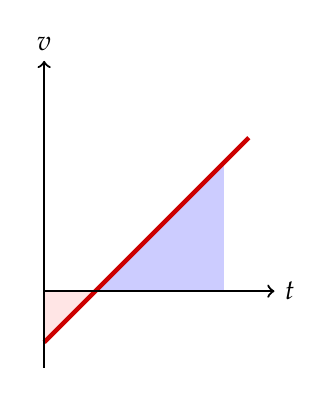
\begin{tikzpicture}[scale=.65]
        \draw[pink!40,fill=pink!40](0,0)--(0,-1)--(1,0)--cycle;
        \draw[blue!20,fill=blue!20](1,0)--(3.5,0)--(3.5,2.5)--cycle;
        \draw[red!80!black,ultra thick](0,-1)--(4,3);
        \draw[->,thick] (0,0)--(4.5,0) node[pos=1,right]{$t$};
        \draw[->,thick] (0,-1.5)--(0,4.5) node[pos=1,above]{$v$};
      \end{tikzpicture}
    \end{center}
    
    \column{.75\textwidth}
    The area under the $v-t$ graph is the displacement $x-x_0$.
    \begin{itemize}
    \item Area \textcolor{blue!20}{\emph{above}} the time axis: $+$
      displacement
    \item Area \textcolor{red!40}{\emph{below}} the time axis: $-$ displacement
    \end{itemize}
    \vspace{.2in}Likewise, the area under the $a-t$ graph is the change in
    velocity $v-v_0$.
  \end{columns}
\end{frame}



%\begin{frame}{Solving Typical Kinematics Problems}
%  
%  \textbf{One object:} the problem provides $3$ of the $5$ variables, and you
%  are asked to find a $4$th one.
%  \begin{itemize}
%  \item Define the positive direction (usually very obvious)
%  \item Apply the correct kinematic equation and solve the problem!
%  \end{itemize}
%
%  \vspace{.2in}\textbf{Two objects:} two objects are in motion. Usually one of
%  them is moving at constant velocity while the other is accelerating.
%  \begin{itemize}
%  \item Time interval $\Delta t$ and displacement $\Delta\mb{x}$ of the two
%    objects are related
%  \item Examples:
%    \begin{itemize}
%    \item Police car chasing a speeder
%    \item Two football players running towards each other
%    \item A person trying to catch the bus
%    \end{itemize}
%  \end{itemize}
%\end{frame}


\section{Projectile Motion}

\begin{frame}{Projectile Motion}
  A \textbf{projectile} is an object that is launched with an initial velocity
  of $\mb{v}_0$ along a parabolic trajectory and accelerates only due to
  gravity.
  \begin{center}
    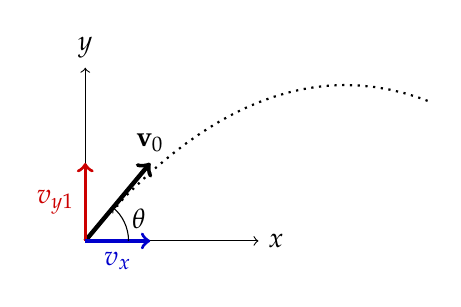
\begin{tikzpicture}[scale=1.1]
      \draw[->](0,0)--(2,0) node[pos=1,right]{$x$};
      \draw[->](0,0)--(0,2) node[pos=1,above]{$y$};
      \draw[dotted,domain=0:4,thick] plot (\x, {1.2*\x-.2*\x*\x});
      \draw[ultra thick,->](0,0)--(.75,.9)node[pos=1,above]{$\mb{v}_0$};
      \draw[very thick,red!80!black,->]
      (0,0)--(0,.9)node[midway,left]{$v_{y1}$};
      \draw[very thick,blue!80!black,->]
      (0,0)--(.75,0)node[midway,below]{$v_x$};
      \draw[->](.5,0)arc(0:52:.5) node[pos=.6,right]{$\theta$};
    \end{tikzpicture}
  \end{center}
  \begin{itemize}
  \item $x$-axis is the \emph{horizontal} direction, with the ($+$) direction
    pointing \emph{forward}
  \item $y$-axis is the \emph{vertical} direction, with the ($+$) direction
    pointing \emph{up}
  \item The reference point is where the projectile is launched
  \item Consistent with the right-handed Cartesian coordinate system
  \end{itemize}
\end{frame}



\begin{frame}{Horizontal ($x$) Direction}
  No acceleration (i.e.\ $a_x=\num{0}$) in the horizontal direction, therefore
  horizontal velocity component is constant. The kinematic equations reduce to:

  \eq{-.2in}{
    x=v_xt=\left[v_0\cos\theta\right] t
  }

  where $x$ is the horizontal position at time $t$, $v_0$ is the
  magnitude of the initial velocity, $v_x=v_0\cos\theta$ is its horizontal
  component.
\end{frame}




\begin{frame}{Vertical ($y$) Direction}
  Constant acceleration due to gravity alone in the vertical direction, i.e.\
  $a_y=-g$. (Acceleration is \emph{negative} due to the way we defined the
  coordinate system.) The important equation is this one:

  \eq{-.2in}{
    y = \left[v_0\sin\theta\right]t-\frac12gt^2
  }

  These two kinematic equations may also be useful:

  \vspace{-.2in}{\Large
    \begin{align*}
      v_y &= \left[v_0\sin\theta\right] -gt\\
      v_y^2&=\left[v_0\sin\theta\right]^2-2gy
    \end{align*}
  }
\end{frame}



\begin{frame}{Solving Projectile Motion Problems}
  Horizontal and vertical motions are independent of each other, but there are
  variables that are shared in both directions, namely:
  \begin{itemize}
  \item Time $t$
  \item Launch angle $\theta$ (above the horizontal)
  \item Initial speed $v_0$
  \end{itemize}
  
  \vspace{.2in}When solving any projectile motion problems
  \begin{itemize}
  \item \emph{Two} equations with \emph{two} unknowns
  \item If an object lands on an incline, there will be a third equation
    describing the relationship between $x$ and $y$
  \end{itemize}
\end{frame}



\begin{frame}{Symmetric Trajectory}
  A projectile's trajectory is symmetric if the object lands at the same height
  as when it launched.
  \begin{itemize}
  \item Time of flight
    \eq{-.1in}{t_\mathrm{max}=\frac{2v_0\sin\theta}{g}}
  \item Range
    \eq{-.1in}{R=\frac{v_0^2\sin(2\theta)}{g}}
  \item Maximum height
    \eq{-.1in}{y_\mathrm{max}=\frac{v_0^2\sin^2\theta}{2g}}
  \end{itemize}
  The angle $\theta$ is measured above the the horizontal.
\end{frame}



\begin{frame}{Maximum Range}
  \eq{-.1in}{R=\frac{v_0^2\sin(2\theta)}{g}}
  
  \begin{itemize}
  \item Maximum range occurs at $\theta=\ang{45}$
  \item For a given initial speed $v_0$ and range $R$, launch angle $\theta$ is
    given by:
    
    \eq{-.2in}{
      \theta_1=\frac{1}{2}\sin^{-1}\left(\frac{Rg}{v_0^2}\right)
    }

    But there is another angle that \emph{gives the same range}!

    \eq{-.2in}{
      \theta_2=\ang{90}-\theta_1
    }
  \end{itemize}
\end{frame}


\section{Relative Motion}

\begin{frame}{Relative Motion}
  \begin{columns}
    \column{.4\textwidth}
    \begin{tikzpicture}[scale=1.3]
      \draw[->](0,0)--(-.5,-.5)
      node[pos=1,left]{$x$}
      node[pos=0,above left]{$C$};
      \draw[->](0,0)--(1,0) node[pos=1,right]{$y$};
      \draw[->](0,0)--(0,1) node[pos=1,above]{$z$};

      \draw[->](2,3)--(1.5,2.5)
      node[pos=1,left]{$x'$}
      node[pos=0,above left]{$B$};
      \draw[->](2,3)--(3,3) node[pos=1,right]{$y'$};
      \draw[->](2,3)--(2,4) node[pos=1,above]{$z'$};

      \fill[red!70!black] (3,1) circle(.03) node[below right]{$A$};
      \draw[very thick,->,blue!70!black](0,0)--(2.98,.998)
      node[midway,below]{$\mb{x}_{AC}$};
      \draw[very thick,->,green!80!black](2,3)--(3,1.03)
      node[midway,right]{$\mb{x}_{AB}$};
    \end{tikzpicture}

    \column{.6\textwidth}
    \fbox{
      \begin{minipage}{.9\textwidth}
        All motion quantities must be measured relative to a frame of
        reference
      \end{minipage}
    }
    \begin{itemize}
    \item Two \textbf{frames of reference} (i.e.\ \textbf{coordinate systems})
      $C(x,y,z)$ and $B(x',y',z')$
    \item Object $\textcolor{red!80!black}{A}$ can be described by the position
      vector $\textcolor{blue!70!black}{\mb{x}_{AC}}$ (position of $A$ relative
      to frame $C$) or $\textcolor{green!80!black}{\mb{x}_{AB}}$ ($A$ relative
      to frame $B$)
      \begin{itemize}
      \item It is clear that $\mb{x}_{AB}$ and $\mb{x}_{AC}$ are different
      \item If the object moves, then $\mb{x}_{AB}$ and $\mb{x}_{AC}$ are
        functions of time
      \end{itemize}
    \item If position depends on the reference frame, then so do velocity and
      acceleration
    \end{itemize}
  \end{columns}
\end{frame}



\begin{frame}{Relative Motion}
  \begin{columns}
    \column{.4\textwidth}
    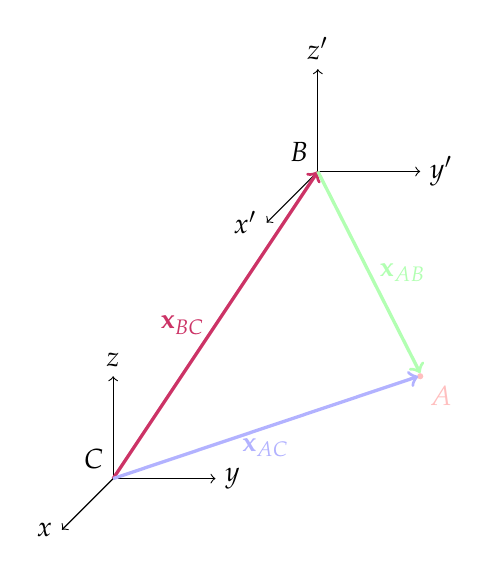
\begin{tikzpicture}[scale=1.3]
      \draw[->](0,0)--(-.5,-.5)
      node[pos=1,left]{$x$}
      node[pos=0,above left]{$C$};
      \draw[->](0,0)--(1,0) node[pos=1,right]{$y$};
      \draw[->](0,0)--(0,1) node[pos=1,above]{$z$};

      \draw[->](2,3)--(1.5,2.5)
      node[pos=1,left]{$x'$}
      node[pos=0,above left]{$B$};
      \draw[->](2,3)--(3,3) node[pos=1,right]{$y'$};
      \draw[->](2,3)--(2,4) node[pos=1,above]{$z'$};
      
      \draw[very thick,->,purple!80](0,0)--(2,3)
      node[midway,left]{$\mb{x}_{BC}$};
      \fill[pink] (3,1) circle(.03) node[below right]{$A$};
      \draw[very thick,->,blue!30](0,0)--(2.98,.998)
      node[midway,below]{$\mb{x}_{AC}$};
      \draw[very thick,->,green!30](2,3)--(3,1.03)
      node[midway,right]{$\mb{x}_{AB}$};
      
    \end{tikzpicture}

    \column{.6\textwidth}
    \begin{itemize}
    \item The relative position of the origins of the two frames of reference
      can is $\mb{x}_{BC}$
      \begin{itemize}
      \item The vector pointing from the origin of frame $C$ to the origin of
        frame $B$
      \item If the two frames are moving relative to each other, then
        $\mb{x}_{BC}$ is a function of time
      \end{itemize}
    \item Without needing vector notations, it should be obvious that

      \eq{-.3in}{
        \textcolor{blue!70!black}{\mb{x}_{AC}}=
        \textcolor{green!80!black}{\mb{x}_{AB}}+
        \textcolor{purple!80}{\mb{x}_{BC}}
        }
    \end{itemize}
  \end{columns}
\end{frame}



\begin{frame}{Relative Motion}
  \begin{columns}
    \column{.4\textwidth}
    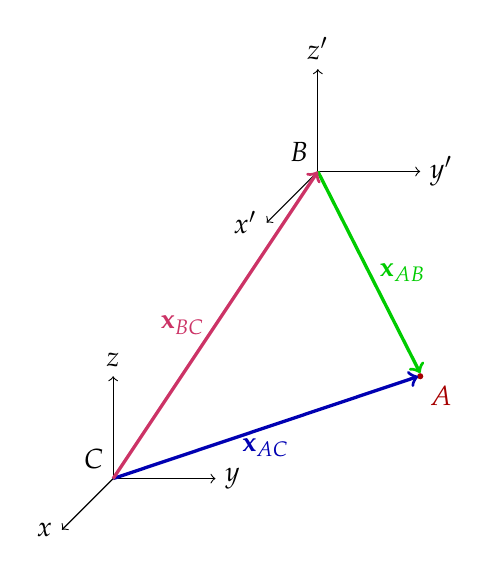
\begin{tikzpicture}[scale=1.3]
      \draw[->](0,0)--(-.5,-.5)
      node[pos=1,left]{$x$}
      node[pos=0,above left]{$C$};
      \draw[->](0,0)--(1,0) node[pos=1,right]{$y$};
      \draw[->](0,0)--(0,1) node[pos=1,above]{$z$};

      \draw[->](2,3)--(1.5,2.5)
      node[pos=1,left]{$x'$}
      node[pos=0,above left]{$B$};
      \draw[->](2,3)--(3,3) node[pos=1,right]{$y'$};
      \draw[->](2,3)--(2,4) node[pos=1,above]{$z'$};

      \fill[red!65!black] (3,1) circle(.03) node[below right]{$A$};
      \draw[very thick,->,blue!70!black](0,0)--(2.98,.998)
      node[midway,below]{$\mb{x}_{AC}$};
      \draw[very thick,->,green!80!black](2,3)--(3,1.03)
      node[midway,right]{$\mb{x}_{AB}$};
      \draw[very thick,->,purple!80](0,0)--(2,3)
      node[midway,left]{$\mb{x}_{BC}$};
    \end{tikzpicture}

    \column{.6\textwidth}
    Assuming that all the position vectors are differentiable in time, then the
    time derivative gives the \textbf{relative velocity}:

    \vspace{-.3in}{\Large
      \begin{align*}
        \frac{d}{dt}\left(\textcolor{blue!70!black}{\mb{x}_{AC}}\right) &=
        \frac{d}{dt}\left(\textcolor{green!80!black}{\mb{x}_{AB}}+
        \textcolor{purple!80}{\mb{x}_{BC}}\right)\\
        \textcolor{blue!70!black}{\mb{v}_{AC}} &=
        \textcolor{green!80!black}{\mb{v}_{AB}}+
        \textcolor{purple!80}{\mb{v}_{BC}}
      \end{align*}
    }

    \vspace{-.2in}Differentiating in time again gives the equation for
    \textbf{relative acceleration}:

    \eq{-.3in}{
      \textcolor{blue!70!black}{\mb{a}_{AC}}=
      \textcolor{green!80!black}{\mb{a}_{AB}}+
      \textcolor{purple!80}{\mb{a}_{BC}}
    }
  \end{columns}
\end{frame}



\begin{frame}{Relative Velocity Example}
  If an airplane ($P$) flies in windy air ($A$) we must consider the velocity
  of the airplane relative to air, i.e.\ $\mb{v}_{PA}$ and the velocity of the
  air relative to Earth $E$, i.e.\ $\mb{v}_{AE}$. The velocity of the airplane
  relative to Earth is therefore

  \eq{-.2in}{
    \mb{v}_{PE}=\mb{v}_{PA}+\mb{v}_{AE}
  }

  \textbf{Simple example:} If an airplane is flying at a constant velocity of
  \SI{253}{km/h} south relative to the air and the air velocity is
  \SI{24}{km/h} east, what is the velocity of the airplane relative to Earth?
\end{frame}



\begin{frame}{Relative Velocity}
  In classical mechanics, the equation for relative motion follows the
  \textbf{Galilean velocity addition rule}:

  \eq{-.25in}{
    \mb{v}_{AC}=\mb{v}_{AB}+\mb{v}_{BC}
  }

  \vspace{-.1in}The velocity of $A$ relative to reference frame $C$ is the
  velocity of $A$ relative to reference frame $B$, plus the velocity of $B$
  relative to $C$. If we add another reference frame $D$, the equation becomes:

  \eq{-.25in}{
    \mb{v}_{AD}=\mb{v}_{AB}+\mb{v}_{BC}+\mb{v}_{CD}
  }
\end{frame}


\begin{frame}{Typical Problems}
  In an AP Physics C exam, questions involving kinematics usually appear in the
  multiple-choice section. The problems themselves are not very different
  compared to the Grade 12 Physics problems, but:
  \begin{itemize}
  \item You have to solve problems faster because of time constraint
  \item You can use $g=\SI{10}{\metre/\second\squared}$
    in your calculations to make your lives    simpler
  \item A lot of problems are \emph{symbolic}, which means that they deal with
    the equations, not actual numbers
  \item Will be coupled with other types (e.g.\ dynamics and rotational) in
    the free-response section
  \item You \emph{will} be given an equation sheet
  \end{itemize}
\end{frame}

\end{document}
